
\begin{frame}
  \LectureNo{10}
  \maketitle
\end{frame}

\begin{frame}{Overview}
  \setcounter{framenumber}{212}
  \tableofcontents
\end{frame}

\section{Rehash}
\begin{frame}{Rehash}
	
	\begin{itemize}%[<+->]
	\itemsep=16pt
	
	\item Propositional logic deals with inferences involving the connectives ``not,'' ``and,'' ``or,'' \dots; \alert{we now move to first-order logic which allows for quantifiers ``for all'' and ``there exists.''}

	\item We start with syntax: modeling target aspects of ordinary language by means of a precise, formal language.
	
\end{itemize}

\end{frame}
		

\section{8. Syntax of First-Order Logic}
\subsection{8.1 First-Order Languages}

\begin{frame}{8.1 First-Order Languages}

	\begin{itemize}%[<+->]
	\itemsep=16pt
		
		\item (8.1.1) Reasoning with quantifiers ``for all'' and ``there is'':
		
		\begin{enumerate}[(1)]
		\setcounter{enumii}{2}
	
		\item This ball is scarlet and everything that's scarlet is red. So, this ball is red.
		
		\item The letter is in the left drawer. So there is something in the left drawer.
	
	\end{enumerate}
	
	\item These arguments are not valid in propositional logic---because the resources of propositional logic are just too limited.
	\[p,q\nvDash r\]
	\[p\nvDash q\]
		
	\item (8.1.2) We need to take into account the \emph{internal grammatical structure} of sentences:
		\[\underbrace{\text{The ball}}_{\text{Term}}~\underbrace{\text{is scarlet}}_{\text{Predicate}}\]
		
	\end{itemize}

\end{frame}

\begin{frame}{Abstraction}

	\begin{itemize}%[<+->]
	\itemsep=16pt
	
		\item The concrete terms and predicates don't matter:
				\begin{enumerate}[(1')]
		\setcounter{enumii}{2}
	
		\item This train is slow and everything that's slow is yellow. So, this train is yellow.
		
		\item The dog is in the car. So there is something in the car.
	
	\end{enumerate}

	\item So, we can abstract away from them:
		
			\begin{itemize}
			
				\item Terms: $t,u,v,\mathellipsis$
				
				\item Predicates: $P,R,Q,\mathellipsis$
			
			\end{itemize}
			
	\item We get:
	
		\begin{itemize}
		
			\item The ball is red $\leadsto$ $P(t)$
			
			\item The letter is in the left drawer $\leadsto$ $R(t,u)$
		
		\end{itemize}

	
	\end{itemize}

\end{frame}

\begin{frame}{Kinds of Terms}

	\begin{itemize}%[<+->]
	\itemsep=16pt
	
		\item (8.1.3) Three kinds of terms in our formal language:
		
		\begin{itemize}
		
			\item \emph{constants} invariantly refer to one specific thing, like the names of people ``Johannes'' or places ``Amsterdam'' ($a,b,c,\mathellipsis$)

			\item \emph{variables} require context to refer, but could potentially refer to anything, like the pronouns ``it'' or ``that''  ($x,y,z,\mathellipsis$)

			\item \emph{functional terms} take `input' from a simpler term and map it to an `output' like ``the birthplace of Hein'' ($f(\mathellipsis),g(\mathellipsis),\mathellipsis$)
		
		\end{itemize}
		
		\item (8.1.4) Note how functions can be \emph{nested}:
		
			\begin{itemize}
			
				\item[] The teacher of both Ada and the teacher of Bob and Cath
				
				\item[] \; $\leadsto$  $f(a,f(b,c))$ 
			
			\end{itemize}
	
	\end{itemize}

\end{frame}

\begin{frame}{The Universal Quantifier}

	\begin{itemize}%[<+->]
	\itemsep=16pt
	
		\item (8.1.6) How to think about quantified sentence structure:
		
		\medskip
		
		\begin{itemize}
		\itemsep=10pt
		\item[] Everything that's scarlet is red.
		\item[$\leadsto$] 
		{\footnotesize
		Every $\underbrace{\text{object}}_{\text{indefinite}}$ is such that if $\underbrace{\text{it}}_{\text{pronoun}}$ is scarlet, then $\underbrace{\text{it}}_{\text{pronoun}}$ is red.
		}
		\item[$\leadsto$] Every $x$ is such that if $x$ is scarlet, then $x$ is red.
		\end{itemize}
		
		\item In symbols, we write this with the \emph{universal quantifier} $\forall$:
		\[
		\forall x(S(x)\to R(x))
		\]

	\end{itemize}

\end{frame}

\begin{frame}{The Existential Quantifier}

	\begin{itemize}%[<+->]
	\itemsep=16pt
	
		\item (8.1.7) A different kind of quantified sentence:
		
		\medskip
		
		\begin{itemize}
		\itemsep=10pt
		\item[] There is something big in the yard.
		\item[$\leadsto$] 
		{\footnotesize
		There is an $\underbrace{\text{object}}_{\text{indefinite}}$ such that $\underbrace{\text{it}}_{\text{pronoun}}$ is big and $\underbrace{\text{it}}_{\text{pronoun}}$ is in the yard.
		}
		\item[$\leadsto$] There is an $x$ such that $x$ is big and $x$ is in the yard.
		\end{itemize}
		
		\item In symbols, we write this with the \emph{existential quantifier} $\exists$:
		\[
		\exists x(B(x)\land Y(x))
		\]

	\end{itemize}

\end{frame}

\begin{frame}{Summary}

	\begin{tabular}{c | l | l}
	Symbol & Name & Reading\\\hline
	$a,b,c,\mathellipsis$ & Constants & Names\\
	$x,y,z,\mathellipsis$ & Variables & Pronouns\\
	$f,g,h, \mathellipsis$ & Function symbols & Functional expressions\\
	$P,Q,R,\mathellipsis$ & Predicate symbols & Properties, relations\\
	$\forall $ & Universal quantifier & every, for all, \dots\\
	$\exists$ & Existential quantifier & there exists, for some, \dots
	\end{tabular}


\end{frame}

\subsection{8.2 Terms and Formulas}
\begin{frame}{8.2 Terms and Formulas}

	\begin{itemize}%[<+->]
	\itemsep=16pt
	
		\item (8.2.1) A \emph{signature} is a structure $\mathcal{S}=(\mathcal{C}, \mathcal{F}, \mathcal{R}, ar)$ such that:
		\begin{enumerate}[(i)]
		
			\item $\mathcal{C}$ is a set of \emph{constant symbols}
			
			\item $\mathcal{F}$ is a set of \emph{function symbols}
			
			\item $\mathcal{R}$ is a set of \emph{predicate symbols}
			
			\item $ar:\mathcal{F}\cup\mathcal{R}\to\mathbb{N}$ is a function that assigns to each function and predicate symbol a fixed natural number, it's \emph{arity}
		\end{enumerate}

	\item (8.2.2) Notation:
	
		\begin{itemize}
		
			\item $R^n\in\mathcal{R}$ means $R\in\mathcal{R}$ with $ar(R)=n$
			\item $f^n\in\mathcal{F}$ means $f\in\mathcal{F}$ with $ar(f)=n$
		
		\end{itemize}
	
	\end{itemize}

\end{frame}

\begin{frame}{(8.2.3) Examples}

	\begin{enumerate}[(i)]
			
				\item $\mathcal{S}_{PA}=(\{0\}, \{S^1, +^2, \cdot^2\}, \alert{\emptyset})$ 
				
				\item $\mathcal{S}_\emptyset=(\alert{\emptyset},\alert{\emptyset},\alert{\emptyset})$
				
				\item $\mathcal{S}_\in=(\{\emptyset\}, \emptyset, \{\in^2\})$
			
			
				\item$\mathcal{S_\ast}=(\{a,b,c\}, \{f^1, g^2\}, \{P^1, R^2\})$			
			\end{enumerate}	
\end{frame}

\begin{frame}{Logical Vocabulary}

	\begin{itemize}%[<+->]
	\itemsep=16pt
	
		\item (8.2.4) The same \emph{logical} vocabulary are always around:
		\begin{enumerate}[(i)]
		
			\item the set of \emph{variables}: $\mathcal{V}=\{x,y,z,\mathellipsis\}$
			
			\item the \emph{sentential operators}: $\neg,\land,\lor,\to,\leftrightarrow$
			
			\item the \emph{identity predicate}: \alert{$=^2$}
			
			\item the \emph{quantifiers}: $\forall,\exists$
			
			\item the \emph{parentheses}: $(,)$.
		
		\end{enumerate}

		\item Note the distinguished, binary \emph{identity predicate} $=$.
		
		\item We write the identity predicate differently (more on that later).
		
			\begin{itemize}
			
				\item[] The birthplace of Ada Lovelace and Bob Ross is the same.
				
				\item[] \; $\leadsto$ $f(a)=f(b)$ \;\; \alert{not} $R(f(a),f(b))$
			
			\end{itemize}
	
	\end{itemize}

\end{frame}

\begin{frame}{The Recursive Definition of Terms}

	\begin{itemize}%[<+->]
	\itemsep=16pt
	
		\item (8.2.5). A particular signature $\mathcal{S}$ generates a recursively defined set $\mathcal{T}$ of \emph{terms}, defined as the smallest set $X$ such that:
		\begin{enumerate}[(i)]
		
			\item \begin{enumerate}[(a)]
			\item $\mathcal{V}\subseteq X$
			\item $\mathcal{C}\subseteq X$
			\end{enumerate}
			\item If $t_1, \mathellipsis, t_n\in X$ and $f\in\mathcal{F}$ with $ar(f)=n$, then $f(t_1, \mathellipsis, t_n)\in X$
	
	\end{enumerate}
	
		\item Terms of a language includes all variables, all constants, and functional combinations of those (and of those, etc.\ldots).
		
	\end{itemize}

\end{frame}

\begin{frame}{(8.2.6) Examples}

	\begin{itemize}
	\itemsep=20pt
			
				\item Terms of $\mathcal{S}_{PA}$: \[S(0),S(S(0)),\mathellipsis\in\mathcal{T}\]\[S(x), S(y), +(0,0), \cdot(0,0), \cdot (Sx, +(0,0)),\mathellipsis\in\mathcal{T}\]	
				
				\item[] This language has its own history and conventions, such as `infix' notation where we write $(0 + S(0))$ for ${+}(0,S(0))$, etc.
					


				\item Terms of $\mathcal{S_\ast}$, assuming that $f^2\in\mathcal{F}$, we have e.g.: \[f(x,x), f(x,y), f(y,x), f(y,y), f(f(x,y), f(y,x)),\mathellipsis\in\mathcal{T}\]
			\end{itemize}


\end{frame}

\begin{frame}{The Recursive Definition of Formulas}

	\begin{itemize}%[<+->]
	\itemsep=16pt
	
			\item (8.2.8). A particular signature $\mathcal{S}$ also generates a recursively defined set $\mathcal{L}$ of \emph{formulas}, the smallest set $X$ such that:
		\begin{enumerate}[(i)]
		
			\item \begin{enumerate}[(a)]
			
				\item If $R^n\in\mathcal{P}$ and $t_1, \mathellipsis, t_n\in \mathcal{T},$ then $R(t_1, \mathellipsis, t_n)\in X$.
				
				\item If $t_1,t_2\in \mathcal{T}$, then $t_1=t_2\in X$
				
				\end{enumerate}
			
			\item \begin{enumerate}[(a)]
			
				\item if $\phi\in X$, then $\neg \phi\in X$
				
				\item if $\phi,\psi\in X$, then $(\phi\circ\psi)\in X$ for $\circ=\land,\lor,\to,\leftrightarrow$
				
				\item if $\phi\in X$ and $x\in \mathcal{V}$, then $Qx\phi\in X$ for $Q=\exists,\forall$
			
			\end{enumerate}
							
		\end{enumerate}
		
		\item (i)(a) and (i)(b) define the \emph{atomic formulas} of the language.
		
		\item $t_1\neq t_2$ is conventional notation for the formula $\neg{t_1=t_2}$

	
	\end{itemize}

\end{frame}

\begin{frame}{(8.2.10.i) Examples}

Formulas in $\mathcal{L}_{PA}$:
					\[x=(S(S(S(S(S(0))))))\]
					\[S(x)=S(S(0))\]
					\[0\cdot S(0)=0\]
					\[\forall x S(x)\neq 0\]
					\[(S(S(0))\cdot S(S(0)))=S(S(S(S(0))))\]
					\[\forall x\forall y(x\neq y\to S(x)\neq S(y))\]
					\[\forall x\forall y(S(x)=y+S(0)\to S(x)=S(y))\]
					\[\forall x\exists yS(x)=y\]


\end{frame}

\begin{frame}{(8.2.10.iv) Examples}

Formulas in $\mathcal{L_\ast}$ over $\mathcal{S_\ast}=(\{a,b,c\}, \{f^1, g^2\}, \{P^1, R^2\})$:
				
				\[R(f(g(a,b)),g(f(a),f(b)))\]
				\[\forall x P(f(a))\]
				\[\forall x(P(a)\to \exists yR(x,y))\]
				\[(\forall xP(x)\land \forall xQ(x))\]
				\[\forall x(P(x)\lor \forall xQ(x))\]
				\[(P(x)\leftrightarrow \forall y\forall xR(x,y))\]

\end{frame}

\begin{frame}{Induction on $\mathcal{L}$}

	\begin{itemize}%[<+->]
	\itemsep=16pt


	\item \textbf{Theorem}.  Let $\Phi$ be a condition on terms. If we can show:
		\begin{enumerate}[(i)]
		
			\item  \begin{enumerate}[(a)]
			
				\item $\Phi(x)$ for all $x\in\mathcal{V}$

				\item $\Phi(a)$ for all $a\in\mathcal{C}$
							
			\end{enumerate}
			
			\item If $\Phi(t_1), \mathellipsis,\Phi(t_n),$ then $\Phi(f(t_1,\mathellipsis,t_n))$ for all $f\in\mathcal{F}$.
		\end{enumerate}
		Then we have shown that $\Phi(t)$ for all $t\in\mathcal{T}$.
	
		\item \textbf{Theorem}. Let $\Phi$ be a condition on formulas. If we can show:
		\begin{enumerate}[(i)]
		
			\item  \begin{enumerate}[(a)]
			
				\item $\Phi(R(t_1,\mathellipsis, t_n))$ for all $R^n\in \mathcal{R}$ and $t_1,\mathellipsis, t_n\in\mathcal{T}$
				
				\item $\Phi(t_1=t_2)$ for all $t_1,t_2\in \mathcal{T}$
			
			\end{enumerate}
			
			\item \begin{enumerate}[(a)]
			
			\item If $\Phi(\psi)$, then $\Phi(\neg\psi)$.

			\item If $\Phi(\psi)$ and $\Phi(\chi)$, then $\Phi((\psi\circ\chi))$, for $\circ=\land,\lor,\to,\leftrightarrow$.
			
			\item If $\Phi(\psi)$, then $\Phi(Qx\psi)$ for $Q=\forall,\exists$.

		
		\end{enumerate}
		\end{enumerate}
		Then we have shown that $\Phi(\psi)$ for all $\psi\in\mathcal{L}$.
	
	\end{itemize}


\end{frame}

\subsection{8.3 Parsing Trees and Occurrences}
\begin{frame}{8.3 Parsing Trees and Occurrences}

	\begin{itemize}%[<+->]
	\itemsep=16pt
	
		\item (8.3.2) We define the parsing tree $T$ operation on terms:

\medskip

\begin{center}
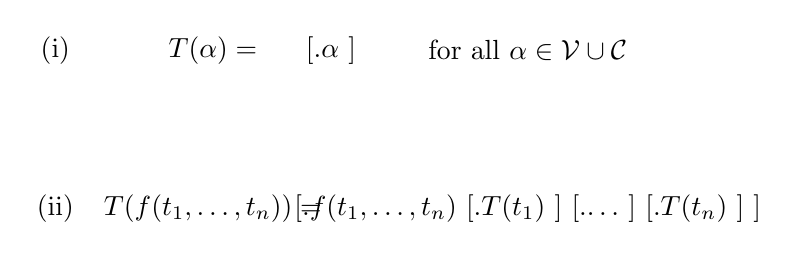
\begin{tikzpicture}
\node at (-2,1) {(i)};

\node at (0,1) {$T(\alpha)=$};
\node at (1.5,1) {\Tree [.$\alpha$ ]};
\node at (4,1) {for all $\alpha\in\mathcal{V}\cup\mathcal{C}$};

\node at (-2,-1) {(ii)};
\node at (0,-1) {$T(f(t_1, \mathellipsis,t_n))=$};
\node at (4,-1) {\Tree [.{$f(t_1, \mathellipsis,t_n)$} [.{$T(t_1)$} ] [.$\mathellipsis$ ] [.{$T(t_n)$} ] ]};

\end{tikzpicture}
\end{center}

	
	\end{itemize}

\end{frame}

\begin{frame}{(8.3.4) Parsing Trees for Formulas}

{\small
\begin{center}
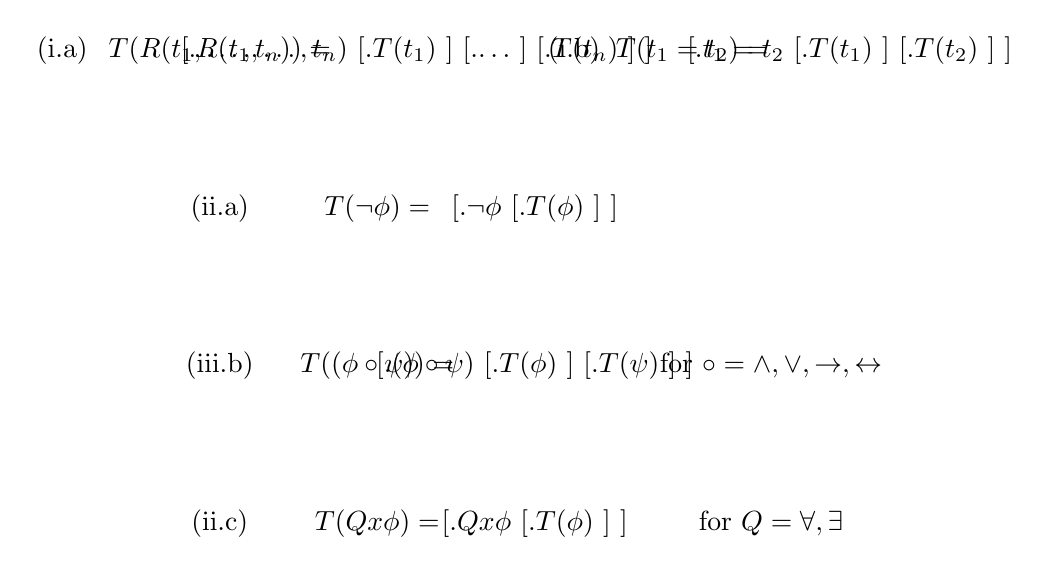
\begin{tikzpicture}
\node at (-4,1) {(i.a)};

\node at (-2,1) {$T(R(t_1, \mathellipsis, t_n))=$};
\node at (0.5,1) {\Tree [.{$R(t_1, \mathellipsis,t_n)$} [.{$T(t_1)$} ] [.$\mathellipsis$ ] [.{$T(t_n)$} ] ]};

\node at (2.5,1) {(i.b)};
\node at (4,1) {$T(t_1=t_2)=$};
\node at (6,1) {\Tree [.$t_1=t_2$ [.$T(t_1)$ ] [.$T(t_2)$ ] ]};

\node at (-2,-1) {(ii.a)};
\node at (0,-1) {$T(\neg \phi)=$};
\node at (2,-1) {\Tree [.$\neg \phi$ [.$T(\phi)$ ] ]};

\node at (-2,-3) {(iii.b)};
\node at (0,-3) {$T((\phi\circ\psi))=$};
\node at (2,-3) {\Tree [.$(\phi\circ\psi)$ [.$T(\phi)$ ] [.$T(\psi)$ ] ]};
\node at (5,-3) {for $\circ=\land,\lor,\to,\leftrightarrow$};


\node at (-2,-5) {(ii.c)};
\node at (0,-5) {$T(Qx \phi)=$};
\node at (2,-5) {\Tree [.$Qx\phi$ [.$T(\phi)$ ] ]};
\node at (5,-5) {for $Q=\forall,\exists$};


\end{tikzpicture}
\end{center}}

\end{frame}

\begin{frame}{(8.3.5) Example of Full Parsing Tree}

\begin{center}
	
	\Tree [.{$\forall x(R(x,g(f(a),f(b)))\to \exists yR(y,y))$} [.{$R(x,g(f(a),f(b)))\to \exists yR(y,y)$} [.{$R(x,g(f(a),f(b)))$} [.$x$ ] [.{$g(f(a),f(b))$} [.$f(a)$ [.$a$ ]  ] [.$f(b)$ [.$a$ ]  ] ] ] [.$\exists yR(y,y)$ [.$R(y,y)$ [.$y$ ]  [.$y$ ] ] ] ] ]
	
	\end{center}

\end{frame}

\begin{frame}{(8.3.7) Example of Stripped Parsing Tree}

\begin{center}
	
	\begin{tabular}{c c c}
	
	\Tree [.{$\forall x(R(x,g(f(a),f(b)))\to \exists yR(y,y))$} [.{$R(x,g(f(a),f(b)))\to \exists yR(y,y)$} [.{$R(x,g(f(a),f(b)))$} [.$x$ ] [.{$g(f(a),f(b))$} [.$f(a)$ [.$a$ ]  ] [.$f(b)$ [.$a$ ]  ] ] ] [.$\exists yR(y,y)$ [.$R(y,y)$ [.$y$ ]  [.$y$ ] ] ] ] ]
	
	&
	
	\Tree [.{$\forall x$} [.{$\to$} [.{$R$} [.$x$ ] [.{$g$} [.$f$ [.$a$ ]  ] [.$f$ [.$a$ ]  ] ] ] [.$\exists y$ [.$R$ [.$y$ ]  [.$y$ ] ] ] ] ]
	
	\end{tabular}
	
	\end{center}

\end{frame}

\begin{frame}{(8.3.9) Naming Nodes}

			\begin{center}
				\Tree [.$\bullet$ [.$\bullet$  [.$\bullet$ [.$\bullet$ ] ] [.$\bullet$ [.$\bullet$ ] [.$\bullet$ ] ] ] ]
			\end{center}

		\medskip
		
		\begin{itemize}
		
		\item The root is always called $r$.

		\item We name other nodes by giving ``directions'' along edges.
		
		\item The first child of $r$ is $( r, 1)$ -- the \emph{only} child in this example.
		
		\item The first child of $( r, 1)$ is called $( r, 1, 1)$.
		
		\item The \emph{second} child of $( r, 1)$ is called $( r, 1, 2)$.
		
		\item And there is no node called $( r, 1, 1, 2)$ in the example above.
		
	\end{itemize}

\end{frame}

\begin{frame}{Occurrences}

{\small
\begin{itemize}%[<+->]
\itemsep=6pt
	
		\item (8.3.10) An expression $\sigma$ \emph{occurs} in a term or formula $\tau$ iff $\sigma$ is the label of some node in the (ordinary or stripped) parsing tree of $\tau$.
	
	\item $R(x,y)$ occurs in $\forall x(R(x,y)\to \exists x\forall y(R(y,x)\land \neg R(x,y)))$.
\smallskip
\begin{center}{\tiny
\begin{tabular}{c}
\begin{tikzpicture}[level distance = 3em]
{\Tree [.$\forall x(R(x,y)\to \exists x\forall y(R(y,x)\land \neg R(x,y)))$
		[.$R(x,y)\to \exists x\forall y(R(y,x)\land \neg R(x,y))$ 
			[.\alert{$R(x,y)$} [.$x$ ] [.$y$ ] ]
			[.$\exists x\forall y(R(y,x)\land \neg R(x,y))$ 
				[.$\forall y(R(y,x)\land \neg R(x,y))$ 
					[.$R(y,x)\land \neg R(x,y)$ 
						[.$R(y,x)$
							[.$y$ ]
							[.$x$ ]
						]	
						[.$\neg R(x,y)$ 
							[.\alert{$R(x,y)$}
								[.$x$ ]
								[.$y$ ]
							]
						]
					]
				]
			]
		]
	]
}
\end{tikzpicture}
\end{tabular}}
\end{center}

	\item An \emph{occurrence} of $\sigma$ in $\phi$ is $(n,\sigma)$ where $n$ is the node of $\sigma$.
	
	\end{itemize}
}

\end{frame}

\subsection{8.4 Free and Bound Variables}
\begin{frame}{8.4 Free and Bound Variables}

	\begin{itemize}%[<+->]
	\itemsep=16pt
	
		\item We use parsing trees to understand quantifiers.
		Motivation: in the formula $\forall x({N}(x)\to {\exists x}R(x,x))$, we want to say that the quantifier $\forall x$ at $r$ `attaches' to $(r,1,1,1,x)$, but \emph{not} to $(r,1,2,1,1,x)$ or $(r,1,2,1,2,x)$.
		
		\begin{center}
		\Tree [.\alert{$\forall x$} [.$\to$ [.${N}$ [.\alert{$x$} ] ] [.${\color{green}\exists x}$ [.$R$ [.{\color{green}$x$} ] [.{\color{green}$x$} ] ] ] ] ]
		\end{center}
	
	\end{itemize}

\end{frame}

\begin{frame}{Variable Binding}

\begin{itemize}%[<+->]
\itemsep=16pt

	\item (8.4.5) Let $( n, x)$ be an occurrence of a variable $x$ in a formula $\phi$ and $( m, Qy)$ an occurrence of a quantifier $Q=\forall,\exists$ in $\phi$. Then, $( n, x)$ is {\it bound} by  $( m, Qy)$ iff
\begin{enumerate}[(i)]
\item $x=y,$
\item there is an downwards path from $m$ to $n,$
\item this path from $m$ to $n$ does not go through a node $k$ such that $( k, Q'x)$ is an occurrence of a quantifier $Q'=\forall,\exists$ in $\phi$.

\end{enumerate}
If a variable occurrence is not bound, we call it \emph{free}.

\end{itemize}

\end{frame}

\begin{frame}{Example (8.4.6.iii)}


\begin{center}{\small
$\forall x(R(x,y)\to \exists x\forall y(R(y,x)\land \neg R(x,y)))$

\vspace{2ex}

\begin{tabular}{c}
\begin{tikzpicture}[level distance = 2em]
{\Tree [.{\color{red}$\forall x$}
		[.$\to$ 
			[.{$R$} [.{\color{red}$x$} ] [.{\color{purple}$y$} ] ]
			[.{\color{green}$\exists x$ }
				[.{\color{blue}$\forall y$} 
					[.$\land$ 
						[.$R$
							[.{\color{blue}$y$} ]
							[.{\color{green}$x$} ]
						]	
						[.$\neg$ 
							[.{$R$}
								[.{\color{green}$x$} ]
								[.{\color{blue}$y$} ]
							]
						]
					]
				]
			]
		]
	]
}
\end{tikzpicture}
\end{tabular}}
\end{center}

\end{frame}

\begin{frame}{Open and Closed Formulas}

	\begin{itemize}%[<+->]
	\itemsep=16pt
	
		\item (8.4.7) $\phi$ is an open formula iff it has occurrences of free variables; otherwise it called a closed formula or \emph{sentence}.
		
		\item (8.4.8) \emph{Examples}:
		
		\begin{itemize}
			
				\item $\forall x(R(x,y)\to \exists x\forall y(R(y,x)\land \neg R(x,y)))$ is an open formula.

			
				\item $\forall x(\exists y \neg R(x,y)\lor (P(x)\to R(c,y)))$ is an open formula.

				\item $\forall x({N}(x)\to {\exists x}R(x,x))$ is a sentence.
			
			\end{itemize}
			
		
		\item Only sentences represent a `complete thought' that receives a definite truth-value. Only sentences can be used in reasoning. We only care about sentences when we analyze arguments.
		
		
	\end{itemize}

\end{frame}

\subsection{8.5 Substitution}
\begin{frame}{8.5 Substitution in Terms}

	\begin{itemize}%[<+->]
	\itemsep=16pt
	
	
		\item (8.5.1) We define a `re-writing' operation $(s)[x:=t]$ as follows (the result of substituting $t$ for all occurrences of $x$ in $s$):
		
		\medskip	
		
		\begin{enumerate}[(i)]
		\itemsep=10pt
			
				\item $(s)[x:=t]=\begin{cases} s & \text{if } s\neq x\\ t & \text{ if }s=x\end{cases}$ for $s\in \mathcal{C}\cup\mathcal{V}$
				
				\item $(f(t_1,\mathellipsis, t_n))[x:=t]=f((t_1)[x:=t], \mathellipsis, (t_n)[x:=t])$
			
			\end{enumerate} 
			
			
	\end{itemize}

\end{frame}

\begin{frame}{8.5 Substitution in Formulas}
	
	\begin{itemize}%[<+->]
	\itemsep=16pt
	
			\item (8.5.2)  We define a `re-writing' operation $(\phi)[x:=t]$ as follows (the result of substituting $t$ for all \emph{free} occurrences of $x$ in $\phi$):
	
		
		\medskip	
		
		\begin{enumerate}[(i)]
		\itemsep=10pt
	
			\item \begin{enumerate}[(a)] 
			
				\item $(R(t_1, \mathellipsis, t_n))[x:=t]=R((t_1)[x:=t], \mathellipsis, (t_n)[x:=t])$
				
				\item $(t_1=t_2)[x:=t]=t_1[x:=t]=t_2[x:=t]$
				
			\end{enumerate}
			
			\item \begin{enumerate}[(a)] 

			\item $(\neg\phi)[x:=t]=\neg(\phi[x:=t])$

			
			\item $((\phi\circ\psi))[x:=t]=((\phi)[x:=t]\circ(\psi)[x:=t])$ for $\circ=\land,\lor,\to,\leftrightarrow$
			
			\item $(Qy\phi)[x:=t]=\begin{cases} Qy(\phi)[x:=t] & \text{if } y\neq x\\ Qy\phi & \text{if }y=x\end{cases}$ for $Q=\forall,\exists$

			\end{enumerate}
	

			\end{enumerate}
	
	\end{itemize}

\end{frame}

\begin{frame}{Example (8.5.4)}

$(\forall x(\exists y \neg R(x,y)\lor (P(x)\to R(c,y))))[y:=c]$
	\begin{align*}
	&=\forall x((\exists y \neg R(x,y)\lor (P(x)\to R(c,y))))[y:=c]\\
	&=\forall x(((\exists y \neg R(x,y)))[y:=c]\lor (((P(x)\to R(c,y))))[y:=c])\\
	&=\forall x((\exists y \neg R(x,y))\lor ((P(x))[y:=c]\to (R(c,y))[y:=c]))\\
	&=\forall x((\exists y \neg R(x,y))\lor (P((x)[y:=c])\to (R((c)[y:=c]), (y)[y:=c])))\\
	&=\forall x(\exists y \neg R(x,y)\lor (P(x)\to R(c,c)))
	\end{align*}

\end{frame}

\subsection{8.6 Formalization}
\begin{frame}{8.6 Formalization}

	\begin{itemize}%[<+->]
	\itemsep=16pt

	\item (8.6.1) The \emph{translation key} interprets the signature:
	
	\begin{enumerate}[(i)]
		
			\item A so-called \emph{domain of discourse}, $D$, which is the set of things we're talking about.
			
			\item For each constant in the signature, a natural language term it formalizes.
			
			\item For each predicate in the signature, a natural language predicate it formalizes.
			
			\item For each function symbol in the language, a natural language expression it formalizes.
			
		\end{enumerate}


\end{itemize}

\end{frame}

\begin{frame}{(8.6.3) Formalization Guidelines $\exists$}

\begin{tabular}{p{6.5cm} c l}
		
		Somebody who's smart exists & $\leadsto$ & $\exists x S(x)$\\

		
		There's somebody who's not smart & $\leadsto$ & $\exists x\neg S(x)$\\

Somebody's smart and somebody's handsome & $\leadsto$ & $\exists xS(x)\land \exists xH(x)$\\

Somebody's smart and handsome & $\leadsto$ & $\exists x(S(x)\land H(x))$\\
 Nobody's both smart and handsome & $\leadsto$ &$\neg\exists x(S(x)\land H(x))$\\
 
 Somebody, who's smart, is handsome & $\leadsto$ & $\exists x(S(x)\land H(x))$
		
		\end{tabular}
		
		\vspace{4ex}
		
		 \[\alert{\exists x(S(x)\to H(x))}\]

\end{frame}

\begin{frame}{(8.6.4) Formalization Guidelines $\forall$}

\begin{tabular}{p{6cm} c l}
		
		Not everybody handsome is smart & $\leadsto$ & $\neg\forall x(H(x)\to S(x))$\\
Everybody who's smart is handsome & $\leadsto$ &$\forall x(S(x)\to H(x))$\\
A person who's smart is handsome & $\leadsto$ &$\forall x(S(x)\to H(x))$\\
Someone who's smart is handsome & $\leadsto$ &$\forall x(S(x)\to H(x))$\\
Everybody's smart and handsome & $\leadsto$ &$\forall x(S(x)\land H(x))$
		\end{tabular}
		
		\vspace{4ex}
		
		\[\alert{\forall x(P(x)\to S(c))\neq \forall xP(x)\to S(c)}\]
		
		\[\alert{\forall x(P(x)\land S(x))\neq \forall x(P(x)\to S(x))}\]

\end{frame}

\begin{frame}{(8.6.5) Formalization Guidelines $x,y,z,\mathellipsis$}

Variables ``are'' pronouns:

\vspace{4ex}

\begin{tabular}{p{6cm} c l}
		He's handsome & $\leadsto$ & $H(x)$\\
		She's handsome and smart & $\leadsto$ & $H(x)\land S(x)$\\
		He's handsome and \emph{he}'s smart & $\leadsto$ & $H(x)\land S(y)$\\
		He's handsome and she's smart & $\leadsto$ & $H(x)\land S(y)$\\
		That's a smart and handsome gal & $\leadsto$ & $H(x)\land S(x)$\\
		
		
		\end{tabular}

\end{frame}

\begin{frame}{(8.6.7) Numerical Quantifiers}

\[\exists xP(x)\tag{Exists$_1$}\]
\[\forall x\forall y(P(x)\land P(y)\to x=y)\tag{At Most$_1$}\]
\[\exists x(P(x)\land \forall y(P(y)\to x=y))\tag{Exactly$_1$}\]

\[\exists x\exists y(P(x)\land P(y)\land x\neq y)\tag{Exists$_2$}\]
\[\forall x\forall y\forall z(P(x)\land P(y)\land P(z)\to x=y\lor x=z\lor y=z)\tag{At Most$_2$}\]
\[\exists x\exists y(P(x)\land P(y)\land \forall z(P(z)\to x=z\lor y=z))\tag{Exactly$_2$}\]
\end{frame}

\begin{frame}{Core Ideas (Lecture Version)}

	\begin{itemize}%[<+->]
	\itemsep=12pt
	
		\item We analyze the inner structure of atomics in f.o. logic.
		
		\item  Terms stand for objects, predicates for properties/relations.
		
		\item Quantifiers allow us talk about things in generality.
		
		\item A signature has constants, function symbols, and predicates.
		
		\item Both terms and formulas are then defined inductively.
		
		\item A formula without free variables is closed/a sentence.
		
		\item We looked at some guidelines for formalization.
					
	\end{itemize}

\end{frame}


\begin{frame}

	\begin{center}
	{\huge\bf Thanks!}
	\end{center}

\end{frame}
